% This is a LaTeX input file.
%
% A '%' character causes TeX to ignore all remaining text on the line,
% and is used for comments like this one.

\documentclass[a4paper]{article}      % Specifies the document class
                             % The preamble begins here.
\title{Asymptotic distributions of two--sample rank statistics for continuous outcomes}  % Declares the document's title.
\author{
Roger B. Newson
\\ Imperial College London
\\ \href{mailto:r.newson@imperial.ac.uk}{r.newson@imperial.ac.uk}
\\ \href{http://www.imperial.ac.uk/nhli/r.newson/}{\textsl{http://www.imperial.ac.uk/nhli/r.newson/}}
}      % Declares the author's name.
%\date{27 April, 2017}      % Deleting this command produces today's date.

\usepackage{graphics}
\usepackage{hyperref}

%
% Set margins
% (which are explained in Figure C3 of LaTeX User's Guide
% and which CAN BE RESET BY EDITORS AT ANY TIME AS FAR AS I CARE!!!!!!!!
% - RBN.)
%
\setlength{\topmargin}{-0.5in}
%\setlength{\headsep}{0.25in}
\setlength{\oddsidemargin}{0in}
\setlength{\evensidemargin}{0in}
\setlength{\textwidth}{6.5in}
\setlength{\textheight}{10in}

%
% Set page style (headers and footers)
%
\pagestyle{myheadings}
\markboth{\textit{Asymptotic distributions of two--sample rank statistics for continuous outcomes}}
{\textit{Asymptotic distributions of two--sample rank statistics for continuous outcomes}}

\begin{document}             % End of preamble and beginning of text.

\maketitle                   % Produces the title.

\section{Introduction}

We assume that there are two potentially infinite sampling sequences of units,
sampled in a mutually independent way from Subpopulations~0 and 1, respectively, of an overall population.
We define outcome random variables $\{ Y_{0i} \}$ and $\{ Y_{1i} \}$ for the $i$th unit sampled from Subpopulations~0 and 1, respectively.
We will assume that Subpopulation~$i$ has a continuous common probability distribution for the $Y_{ij}$,
with cumulative distribution function $F_i(\cdot)$ and probability density function $f_i(\cdot)$.
For $h\in \{0,1\}$ and $i$ a positive integer,
define $X_{hi}=h$, so that the ordinal $X$--variable indicates membership of the Subpopuation 1,
rather than the Subpopulation 0.
From these sequences, we may take finite samples (Subsample~0 and Subsample~1),
containing units corresponding to the first $N_0$ and $N_1$ positive integers, respectively,
and calculate sample statistics to estimate population parameters, to compare the two subpopulations.

The population parameters that we aim to estimate here are Somers'~$D$, Harrell's~$c$, the Hodges--Lehmann percentile pairwise differences,
and the differences between the subpopulation percentiles.
All of these parameters can be estimated, with sample point estimates and confidence limits, using rank (or ``nonparametric'') methods,
and are discussed in Newson (2002)\cite{newson2002}, or in Bonett and Price (2002)\cite{bonett2002}.
The subsequent sections will define each of these parameters,
and their sample estimates,
and discuss the asymptotic distributions of these sample estimates.
All of these estimates are governed by versions of the the Central Limit Theorem,
and are asymptotically Normally distributed as the smaller of the two subsample sizes becomes large,
with asymptotic variances depending on the $F_i(\cdot)$ and the $f_i(\cdot)$.
Note that we will not necessarily assume that the two subpopulations are equally variable,
although this was often done in the past, to avoid needing computers.
(See, for example, Hodges and Lehmann (1963)\cite{hodges1963} and Lehmann (1963)\cite{lehmann1963}.)

\section{Somers'~$D$ and Harrell's~$c$}

The parameter Somers'~$D$ was introduced by Somers (1962)\cite{somers1962}.
In this two--sample case, it is defined as
\def\sign{{\rm sign}}
\def\Pr{{\rm Pr}}
\begin{equation}
D(Y|X) \quad = \quad E [ \, \sign(Y_{1k} - Y_{0j}) \, \sign(X_{1k \, } - X_{0j}) ] \quad = \quad \Pr(Y_{0j}<Y_{1k}) - \Pr(Y_{0j}>Y_{1k}),
\label{eq:eqseq1}
\end{equation}
assumed to have the same value for all positive integers $j$ and $k$.
An equivalent parameter is Harrell's~$c$ (Harrell \textit{et al.}, 1982)\cite{harrell1982},
defined in this two--sample case as
\begin{equation}
c(Y|X) \quad = \quad [ \, D(Y|X)+1 \, ]/2 \quad = \quad \Pr(Y_{0j}<Y_{1k}) + {1\over 2} \Pr(Y_{0j}=Y_{1k}),
\label{eq:eqseq2}
\end{equation}
equal simply to $\Pr(Y_{0j}<Y_{1k})$ if the $Y$--variables are sampled from continuous distributions,
which of course exist only in theoretical statistics.
Both of these population parameters are estimated using sample statistics.
In the case of Somers'~$D$, the point estimate, for sample numbers $N_0$ and $N_1$, is
\begin{equation}
\hat D_{N_0,N_1}(Y|X) \quad = \quad {1\over{N_0 N_1}} \sum_{j=1}^{N_0} \sum_{k=1}^{N_1} \sign(Y_{1k} - Y_{0j})
\quad = \quad {1\over{N_0 N_1}} \sum_{j=1}^{N_0} \sum_{k=1}^{N_1} [ \, I(Y_{0j} < Y_{1k}) - I(Y_{1k}<Y_{0j}) \, ],
\label{eq:eqseq3}
\end{equation}
where $I(Q)$, for a proposition $Q$, is the indicator function, equal to 1 if $Q$ is true and to 0 if $Q$ is false.
In the case of Harrell's~$c$, the point estimate is
\begin{equation}
\hat c_{N_0,N_1}(Y|X) \quad = \quad [ \, \hat D_{N_0,N_1}(Y|X)+1 \, ]/2
\quad = \quad {1\over{N_0 N_1}} \sum_{j=1}^{N_0} \sum_{k=1}^{N_1} [ \, I(Y_{0j} < Y_{1k}) + {1\over 2}I(Y_{1k}=Y_{0j}) \, ],
\label{eq:eqseq4}
\end{equation}
equal to $(N_0 N_1)^{-1}\sum_{j=1}^{N_0} \sum_{k=1}^{N_1} I(Y_{0j} < Y_{1k})$ if the $Y$--variables are continuous.
Note that both of these statistics are two--sample generalized $U$--statistics in the terminology of Chapter~5
of Serfling (1980)\cite{serfling1980}. In that terminology, the respective kernels of Somers'~$D$ and Harrell's~$c$ are
\begin{equation}
h_D(y_0,y_1) \quad = \quad \sign(y_1-y_0), \quad h_c(y_0,y_1) \quad = \quad I(y_0<y_1) + {1\over 2} I(y_0=y_1),
\label{eq:eqseq5}
\end{equation}
where the second term of the kernel for Harrell's~$c$ is zero for continuous variables.

From this point, we will work with Harrell's~$c$, assume that the $Y_{ij}$ are continuous variables,
and define the kernels and $U$--statistics using the distribution of the underlying uniformly distributed variables
\begin{equation}
U_{ij} \quad = \quad F_i(Y_{ij}),
\label{eq:eqseq6}
\end{equation}
which are mutually independent and have an identical uniform distribution with minimum 0 and maximum 1.
The kernel for Harrell's~$c$ in terms of the $U_{ij}$ is then defined as
\begin{equation}
g(u_0,u_1) \quad = \quad h_c\left[ F_0^{-1}(u_0),F_1^{-1}(u_1) \right] \quad = \quad I\left[ F_0^{-1}(u_0)<F_1^{-1}(u_1) \right].
\label{eq:eqseq7}
\end{equation}
To derive the asymptotic  distribution of $\hat c_{N_0,N_1}(Y|X)$,
we use the methods of Chapter~5 of Serfling (1980)\cite{serfling1980}.
We start by defining the conditional expectations of this kernel,
given values in the interval $(0,1)$ for the $U_{ij}$ in the two subsamples,
as
\begin{equation}
\begin{array}{rcl}
\bar g_0(u) &\quad = \quad& E\left[ \, g(u,U_{1i}) \, \right] \quad = \quad 1 - F_1\left[ \, F_0^{-1}(u) \, \right] , \\
\bar g_1(u) &\quad = \quad& E\left[ \, g(U_{0i},u) \, \right] \quad = \quad F_0\left[ \, F_1^{-1}(u) \, \right] .
\end{array}
\label{eq:eqseq8}
\end{equation}
Note that the two functions $\bar g_0(\cdot)$ and $\bar g_1(\cdot)$ are inversely related,
in that, for $u\in (0,1)$,
\begin{equation}
\bar g_1^{-1}(u) \quad = \quad  1-\bar g_0(u), \quad \bar g_0^{-1}(u) \quad = \quad  \bar g_1(1-u).
\label{eq:eqseq9}
\end{equation}
Note, also, that, in the terminology of diagnostic tests,
the $\bar g_i(\cdot)$ can be defined in terms of the sensitivity and specificity
of a diagnostic test for membership of Subpopulation~1 instead of Subpopulation~0,
defined by assuming that units with $Y$--values above a critical value are members of Subpopulation~1,
and that units with $Y$--values below that critical value are members of Subpopulation~0.
(If the $Y_{ij}$ are continuous, then the probability of a $Y$--value equal to the critical value is zero.)
\def\sens{{\rm sens}}
\def\spec{{\rm spec}}
\def\ycrit{{y_{\rm crit}}}
If we define sensitivity and specificity for a critical value $\ycrit$ respectively as
\begin{equation}
\sens(\ycrit) \quad = \quad 1-F_1(\ycrit) , \quad \spec(\ycrit) \quad = \quad F_0(\ycrit) ,
\label{eq:eqseq10}
\end{equation}
then, for $u\in (0,1)$, we have the equalities
\begin{equation}
\bar g_0(u) \quad = \quad \sens\left[ \, F_0^{-1}(u) \, \right] , \quad  \bar g_1(u) \quad = \quad \spec\left[ \, F_1^{-1}(u) \, \right] .
\label{eq:eqseq11}
\end{equation}
This implies that the mean, variance and other moments of $\sens(Y_{0j})$ are equal to the corresponding moments of $\bar g_0(U_{0j})$,
and that the mean, variance and other moments of $\spec(Y_{1j})$ are equal to the corresponding moments of $\bar g_1(U_{1j})$.
The $\bar g_i(U_{ij})$ are conditional expectations of the kernels $g(U_{0j},U_{1k})$,
and therefore have the common expectation
\begin{equation}
E\left[ \bar g_0(U_{0j}) \right] \quad = \quad c(Y|X) \quad = \quad E\left[ \bar g_1(U_{1j}) \right].
\label{eq:eqseq12}
\end{equation}
The sampling distribution of $\hat c_{N_0,N_1}(Y|X)$ converges, as $\min(N_1,N_2) \rightarrow \infty$, to a Normal form,
with a variance that converges in ratio to the expression
\begin{equation}
N_0^{-1}V\left[ \, \bar g_0(U_{0j}) \, \right] \quad + \quad N_1^{-1}V\left[ \, \bar g_1(U_{1j}) \, \right] ,
\label{eq:eqseq13}
\end{equation}
where $V[\cdot]$ denotes variance.

The expression (\ref{eq:eqseq13}) can be used in approximate power calculations for Harrell's~$c$, and therefore for Somers'~$D$,
whose variance is derived simply by quadrupling the variance of Harrell's~$c$.
To do this, we must specify a model for the $F_i(\cdot)$, to be assumed in the power calculations,
and then calculate the $V[\bar g_i(U_{ij})]$ using the expressions
\begin{equation}
V\left[ \, \bar g_i(U_{ij}) \, \right] \quad = \quad \int_0^1 \left[ \, \bar g_i(u) - c(Y|X) \, \right]^2 du ,
\label{eq:eqseq14}
\end{equation}
which can be calculated numerically, if we can specify a value for $c(Y|X)$
and functional forms for the $F_i(\cdot)$ to be used in the formulas (\ref{eq:eqseq8}).
The numerical integration results for (\ref{eq:eqseq14}) will probably be fairly stable,
given that we are integrating a function whose magnitude is bounded above by 1 over the unit interval.
Typically, when carrying out power calculations, we assume a ``toy model'',
such as a homoskedastic Normal or shifted exponential model,
and hope that this model will produce calculations of power and sample size that are not too greatly in error,
and use rank methods as an insurance policy, in case our ``toy model'' is not exactly true.

\subsection{Example: Harrell's~$c$ between Normal subpopulations}

One possible ``toy model'' is the Normal model, which assumes that the $F_i(\cdot)$ belong to Normal subpopulation distributions,
with means $\mu_0$ and $\mu_1$, and standard deviations (SDs) $\sigma_0$ and $\sigma_1$, respectively.
Under these assumptions, Harrell's~$c$ is given by
\begin{equation}
c(Y|X) \quad = \quad \Phi\left( {{\mu_1 - \mu_0}\over{\sqrt{\sigma_0^2 + \sigma_1^2}}} \right)
\quad = \quad \Phi\left[ {(\mu_1 - \mu_0)/\sigma_0}\over{\sqrt{1 + (\sigma_1/\sigma_0)^2}} \right],
\label{eq:eqseq15}
\end{equation}
where $\Phi(\cdot)$ denotes the standard Normal cumulative distribution function.
Note that Harrell's~$c$ depends only on the difference between the means (expressed in units of the SD of Subpopulation~0)
and on the ratio of the Subpopulation~1 SD to the Subpopulation~0 SD.

\begin{figure}[tb]
\caption{Sensitivity and specificity under 25 combinations of mean difference and standard deviation ratio.}
\label{figure:figseq1}
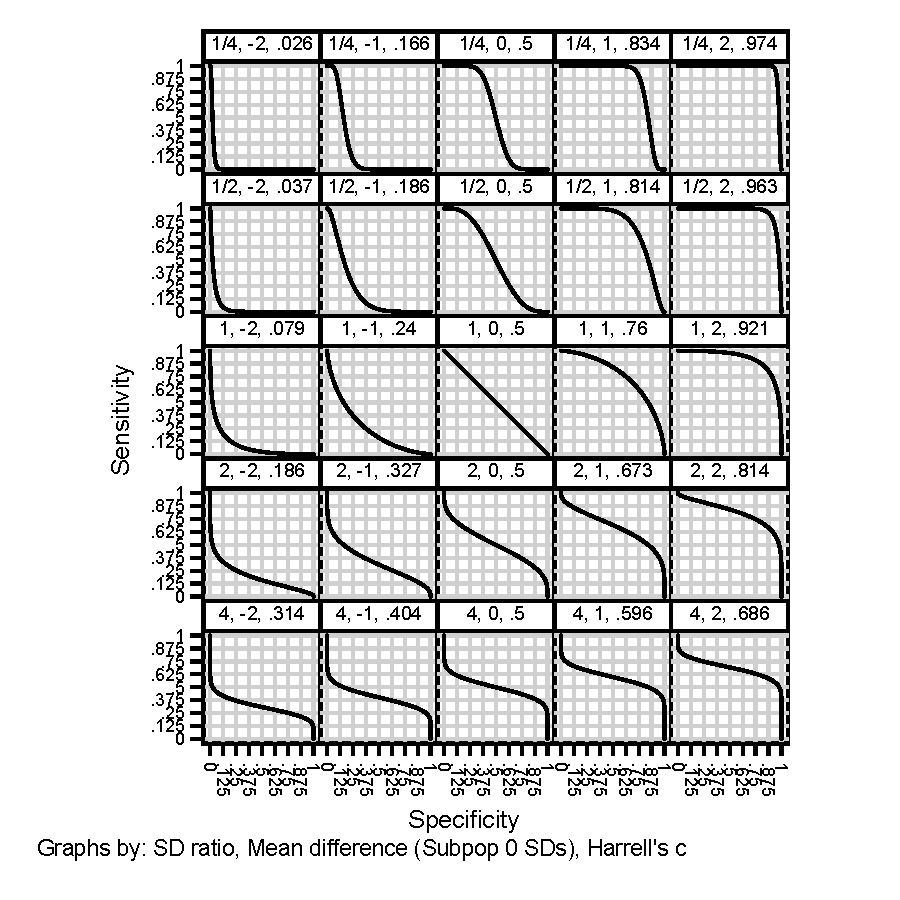
\includegraphics{senspec2.pdf}
\end{figure}

Figure~\ref{figure:figseq1} illustrates the distributions of $\bar g_0(U_{0j})$ and $\bar g_1(U_{1j})$ under 25 scenarios,
corresponding to all possible combinations of 5 mean differences (-2, -1, 0, 2 and 1 Subpopulation~0 SDs)
and 5 SD ratios $\sigma_1/\sigma_0$ (1/4, 1/2, 1, 2 and 4).
The subgraphs correspond to these scenarios,
and are arrayed with rows corresponding to the SD ratios and columns corresponding to the mean differences.
For each subgraph, the value of Harrell's~$c$ is also given in the subtitle.
In each subgraph, the points on the line correspond to candidate critical $Y$--values for use in a diagnostic test,
the vertical axis gives the sensitivity, and the horizontal axis gives the specificity.
Under each scenario,
the population distribution of $\bar g_0(U_{0j})$ can be simulated by sampling points at random from the horizontal specificity axis
and recording the corresponding sensitivity,
and the population distribution of $\bar g_1(U_{1j})$ can be simulated by sampling points at random from the vertical sensitivity axis
and recording the corresponding specificity.
The area under the sensitivity--specificity curve for each scenario is equal to the Harrell's~$c$ for that scenario,
and is discussed as a measure of diagnostic power in Hanley and McNeil (1982)\cite{hanley1982}.
Note that the area under the sensitivity--specificity curve increases progressively between the subgraphs within each row of the graph,
as the mean difference $(\mu_1-\mu_0)/\sigma_0$ increases.

The slope of the sensitivity--specificity curve is negative,
and is equal, at each point, to minus the likelihood ratio $f_1(\ycrit)/f_0(\ycrit)$
of the corresponding candidate critical $Y$--value $\ycrit$.
Note that the subgraphs in the third row, corresponding to a SD ratio of 1,
all have sensitivity--specificity curves that are either convex or concave,
corresponding to a monotonic likelihood ratio,
whereas the subgraphs in the other rows, corresponding to other SD ratios,
all have sigmoid sensitivity--specificity curves,
corresponding to non--monotonic likelihood ratios.
Note, also, that, in each column of the graph (corresponding to a mean difference),
$\bar g_0(U_{0j})$ (corresponding to the vertical axis) becomes progressively less variable as the SD ratio becomes higher,
whereas $\bar g_1(U_{1j})$ (corresponding to the horizontal axis) becomes progressively more variable as the SD ratio becomes higher.
The central subgraph in the third row and the third column corresponds to the case where the subpopulations have equal means and standard deviations,
implying that both $\bar g_0(U_{0j})$ and $\bar g_1(U_{1j})$ are distributed uniformly over the unit interval.
This scenario is a case of the null hypothesis tested by the two--sample Wilcoxon test,
under which the asymptotic variance expression (\ref{eq:eqseq13}) for Harrell's~$c$ is equal to $(N_0^{-1} + N_1^{-1})/12$,
as proved in Chapter~5 of Serfling (1980)\cite{serfling1980}.

\subsection{Power calculations for Harrell's~$c$ using the Normal model}

A statistician may be asked to do power calculations for estimating Harrell's~$c$.
For example, a medical colleague might ask a statistician to compute a power curve for the power to detect a high level of discriminating power
for a newly--developed diagnostic test score.
The null hypothesis may be either a hypothesis of no predictive power at all (corresponding to a Harrell's~$c$ of 0.5 or a Somers'~$D$ of 0),
or a hypothesis of an inferior non--zero level of predictive power (corresponding to a Harrell's~$c$ of 0.6 or a Somers'~$D$ of 0.2).
A statistician's natural response may be to use the Normal model to do the power calculations.
And the statistician may be under pressure to produce these calculations in a hurry,
necessitating a quick and dirty solution which is not far wrong.

The 5 quantities featuring in power calculations (each of which can be calculated from the other 4)
are the power, the significance level (or alpha),
the detectable difference (or delta), the sample size,
and the standard deviation of the influence function.
The latter quantity is defined in Newson (2004)\cite{newson2004}
as the product of the standard error of the sample parameter estimate and the square root of the sample size,
and is equal to the common standard deviation, in the power calculations for an equal--variance $t$--test.
For the two--sample Harrell's~$c$, the asymptotic value of this may be defined, using (\ref{eq:eqseq13}),
as
\def\sigmainf{{\sigma_{\rm inf}}}
\begin{equation}
\sigmainf\left[\hat c(Y|X)\right] \, = \, \sqrt{ p_0^{-1}V\left[ \, \bar g_0(U_{0j}) \, \right] \quad + \quad p_1^{-1}V\left[ \, \bar g_1(U_{1j}) \, \right] } ,
\label{eq:eqseq35}
\end{equation}
where $\hat c(Y|X)$ iss the sample estimate of Harrell's~$c$, $p_0=N_0/(N_0+N_1)$ and $p_1=N_1/(N_0+N_1)$ are the proportions of individuals in Subsample~0 and Subsample~1,
respectively. This may be rewritten in terms of the sample ratio (or odds) $\omega_1=p_1/p_0=p_1/(1-p_1)$ as
\begin{equation}
\sigmainf\left[\hat c(Y|X)\right]
\, = \,
\sqrt{ (1+\omega_1)V\left[ \, \bar g_0(U_{0j}) \, \right] \quad + \quad {{1+\omega_1} \over \omega_1} V\left[ \, \bar g_1(U_{1j}) \, \right] } \, .
\label{eq:eqseq36}
\end{equation}
Given 2 Normal subpopulations with means $\mu_0$ and $\mu_1$ and standard deviations $\sigma_0$ and $\sigma_1$,
this quantity can be calculated by computing $V\left[ \bar g_0(U_{0j}) \right]$ and $V\left[ \bar g_1(U_{1j}) \right]$
by numerical solution of (\ref{eq:eqseq14}), using the expression for $c(Y|X)$ in (\ref{eq:eqseq15}).
As pointed out in Chapter~5 of Serfling (1980)\cite{serfling1980},
the numerical integration is not really necessary if the means and variances are equal,
because then we have  $V\left[ \bar g_0(U_{0j}) \right] = V\left[ \bar g_1(U_{1j}) \right] =1/12$.
However, in the more general case, the means, the variances or both may be unequal.
We must therefore either do some numerical integration to compute (\ref{eq:eqseq14}),
or avoid this programming work by using a variance--stabilizing transformation.
A good candidate variance--stabilizing transformation for Harrell's~$c$ is probably its quarter--logit
\def\logit{{\rm logit}}
\begin{equation}
0.25 \, \logit \left[ c(Y|X) \right],
\label{eq:eqseq37}
\end{equation}
which is equivalent to transforming Somers'~$D(Y|X)$ using the hyperbolic arctangent or Fisher's~$z$ transformation,
as recommended in Edwardes (1995)\cite{edwardes1995}.
The derivative of the quarter--logit with respect to Harrell's~$c$ is
\begin{equation}
{d \over {d c(Y|X)}} 0.25 \, \logit \left[ c(Y|X) \right] = 0.25 \left( { 1 \over {c(Y|X)} } + { 1 \over {1-c(Y|X)} } \right) ,
\label{eq:eqseq38}
\end{equation}
which is 1 under the null hypothesis $c(Y|X)=0.5$.
The asymptotic standard deviation of the influence function for the quarter--logit is therefore
\begin{equation}
\sigmainf\left\{ 0.25 \, \logit \left[ \hat c(Y|X)\right] \right\}
\, = \,
0.25 \left( { 1 \over {c(Y|X)} } + { 1 \over {1-c(Y|X)} } \right)
\sqrt{ (1+\omega_1)V\left[ \bar g_0(U_{0j}) \right] \, + \, {{1+\omega_1} \over \omega_1} V\left[ \bar g_1(U_{1j}) \right] } .
\label{eq:eqseq39}
\end{equation}
If a statistician is working under pressure, then the statistician might be tempted to save programming time
by assuming the standard deviations of the influence functions are equal to their values
under the null hypothesis that the means and variances are both equal.
The null value of the standard deviation of the influence function, under that hypothesis, is
\begin{equation}
\sigmainf\left\{ 0.25 \, \logit \left[ \hat c(Y|X)\right] \right\}
\, = \,
\sigmainf\left[\hat c(Y|X)\right]
\, = \, 
\sqrt{ {{1+\omega_1} \over 12 } \, + \, {{1+\omega_1} \over {12 \omega_1}} } .
\label{eq:eqseq40}
\end{equation}
This simplifying approximation is equivalent to assuming that there exists an unspecified monotonic transformation,
which transforms the distribution of our test score to a variable $Y$,
which is Normally distributed with equal variances in the two subpopulations to be discriminated,
and that the variance--stabilizing quarter--logit transformation of Harrell's~$c$
stabilizes the variance of the sample Harrell's~$c$ perfectly.
If we can make this incredible--sounding assumption,
then we need only worry about the subsample--size ratio $\omega_1$.

\begin{figure}[tb]
\caption{Ratios between computed and null SDs of influence functions.}
\label{figure:figseq3}
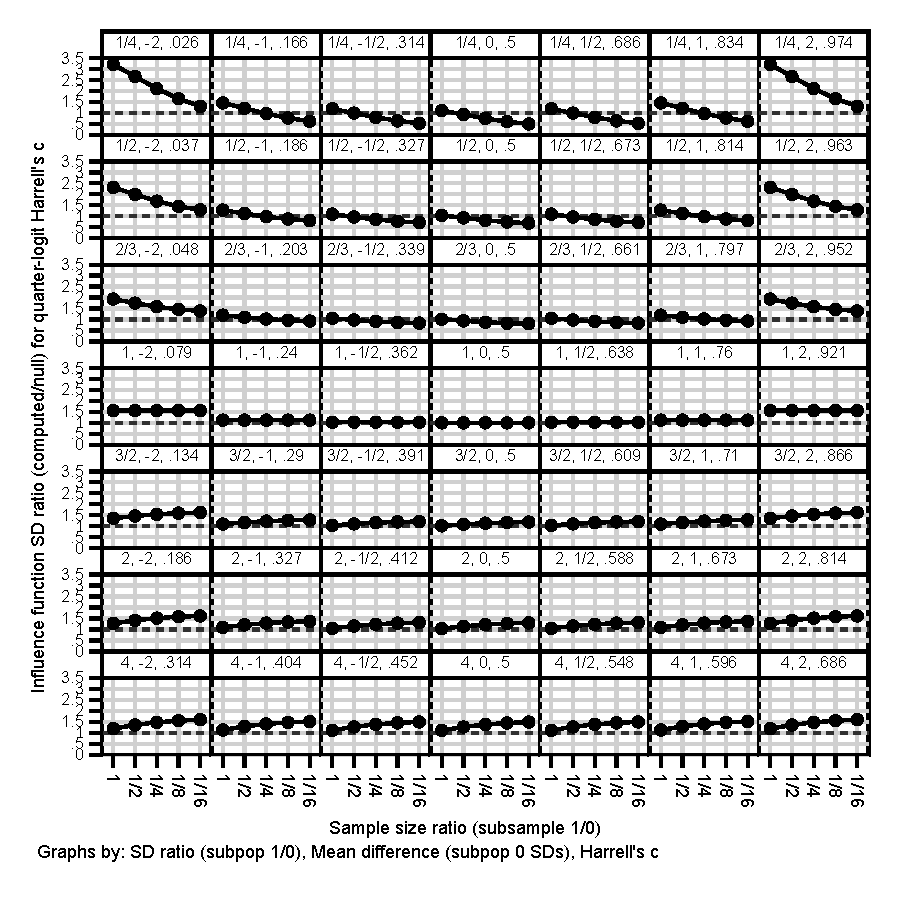
\includegraphics{sdinf1_4.pdf}
\end{figure}

How much damage might be done by using this incredible assumption?
Figure~\ref{figure:figseq3} is a graph matrix, showing the impact of this assumption under a range of scenarios.
The rows of the graph matrix correspond to 7 standard--deviation ratios $\sigma_1/\sigma_0$
(1/4, 1/2, 2/3, 1, 3/2, 2 and 4)
between Subpopulations 1 and 0.
The columns of the graph matrix correspond to 7 possible mean differences $(\mu_1-\mu_0)/\sigma_0$
(-2, -1, -1/2, 0, 1/2, 1 and 2)
between Subpopulations 1 and 0,
expressed in units of the standard deviation of Subpopulation 0.
Each of the 49 combinations of the 7 SD ratios and the 7 mean differences
is specified in its subgraph title,
together with the value of Harrell's~$c$ for that combination of SD ratio and mean difference,
as specified by (\ref{eq:eqseq15}).
The horizontal axis of each graph represents the sample--size ratio
between Subsample~1 (a smaller subsample from Subpopulation~1)
and Subsample~0 (a larger subsample from Subpopulation~0).
And the vertical axis of each graph represents the ratio between the asymptotic SD of the influence function
for the quarter--logit of Harrell's~$c$,
calculated using (\ref{eq:eqseq39}),
and the assumed asymptotic SD of the same influence function,
calculated as the null SD of the influence function,
using the over--simplifying assumption of (\ref{eq:eqseq40}).
This ratio will be 1 if the over--simplifying assumption of (\ref{eq:eqseq40}) is correct,
and close to 1 if it is not far from the truth.
The ratio of 1 is indicated by a horizontal dashed reference line on the vertical axis.

We see that, in the middle row of the graph matrix (corresponding to an SD ratio of 1 between the 2 subpopulations),
the ratio between the calculated and null SDs of the influence function is close to 1
if the mean difference is between -1 and 1 SDs.
And, in the middle 3 rows of the graph
(corresponding to an SD ratio between 2/3 and 3/2),
the ratio between the calculated and null SDs of the influence function
is not radically different from 1.
Outside the range of between--subpopulation SD ratios from 2/3 to 3/2,
and outside the range of between--population mean differences between -1 and 1 Subpopulation 0 SDs,
the over--simplifying null--SD assumption is tested to destruction,
with calculated and null SDs of the influence function
frequently separated by ratios far from 1.
The approximation of (\ref{eq:eqseq39}) by (\ref{eq:eqseq40}) has therefore been tested to destruction.
\textit{However}, we see that, if the subpopulation SDs are not radically different,
and if the Harrell's~$c$ is not outside the range from 0.3 to 0.7,
then the simplifying assumption of (\ref{eq:eqseq40})
should produce power estimates that are less approximate than we had any right to expect.
\textit{So}, if we are planning to measure the discrimination power of a novel biomarker or test score using Harrell's~$c$,
then the incredible--looking formula (\ref{eq:eqseq40}) will produce power calculations not far from the truth,
at least if there exists a transformation that transforms the biomarker or test score to a distribution
that is Normal, with similar variances, in each of the 2 subpopulations between which we want to discriminate.
And, if no such transformation exists,
then we might expect our biomarker or test score to have problems with a non--monotonic likelihood ratio.

\section{Hodges--Lehmann percentile differences}

The pairwise differences between the outcomes in Subsamples~1 and 0 are defined as
\begin{equation}
\Delta_{jk} \quad = \quad Y_{1j} - Y_{0k} ,
\label{eq:eqseq16}
\end{equation}
for positive integers $j$ and $k$,
and are identically distributed, although not statistically independent.
Their common continuous density function, and distribution function, are given by
\begin{equation}
\begin{array}{rcl}
f_\Delta(b) &\quad = \quad& \int_{-\infty}^{\infty} f_1(z) f_0(z-b) dz , \\
F_\Delta(b) &\quad = \quad& \int_{-\infty}^b f_\Delta(b') db' .
\end{array}
\label{eq:eqseq17}
\end{equation}
Note that, for each $b$, we have
\begin{equation}
F_\Delta(b) \quad = \quad \Pr(Y_{1j}-Y_{0k} \le b) \quad = \quad \Pr(Y_{1j}-bX_{1j} \le Y_{0k}-bX_{0k}) \quad = \quad 1 - c(Y-bX|X),
\label{eq:eqseq18}
\end{equation}
where $c(Y-bX|X)$ is a Harrell's~$c$ parameter, defined analogously to $c(Y|X)$ in (\ref{eq:eqseq2}).

For $q\in (0,1)$, a $100q$th Hodges--Lehmann percentile pairwise difference $\beta_q$ between Subpopulations~1 and 0
is defined as a solution in $b$ to the equation
\begin{equation}
0 \quad = \quad F_\Delta(b) - q \quad = \quad 1 - c(Y-bX|X) - q,
\label{eq:eqseq19}
\end{equation}
which is unique if $F_\Delta(\cdot)$ is assumed to be strictly monotonically increasing,
as we will do from this point.
In the terminology of Chapter~5 Serfling (1980)\cite{serfling1980},
the parameter $1-c(Y-bX|X)-q$ is a Hoeffding regular functional for each $b$ and $q$,
and can be estimated, in a pair of samples of $N_0$ and $N_1$,
by the corresponding $U$--statistic $1-\hat c_{N_0,N_1}(Y-bX|X)-q$.
This estimate can be substituted into (\ref{eq:eqseq19}) to derive a consistent sample estimate
$\hat\beta_{q,N_0,N_1}$,
which is a hybrid between the $U$--statistics and $M$--estimates of Chapters~5 and 7, respectively,
of Serfling (1980)\cite{serfling1980}.
The estimate for $q=0.5$ is known as the sample Hodges--Lehmann median difference,
and was introduced by Hodges and Lehmann (1963)\cite{hodges1963} and Lehmann(1963)\cite{lehmann1963}.
More general cases are discussed in Newson (2006)\cite{newson2006}.

The asymptotic distribution of $\hat\beta_{q,N_0,N_1}$, as $\min(N_0,N_1) \rightarrow \infty$,
is derived as follows,
by analogy to the case for $M$--estimates discussed in Chapter~7 of Serfling (1980).
We first differentiate the expression (\ref{eq:eqseq19}) with respect to $b$
to obtain the derivative
\begin{equation}
{d\over{db}}\left[ \, 1 - c(Y-bX|X) - q \, \right] \quad = \quad {d\over{db}}\left[ \, F_\Delta(b) - q \, \right] \quad = \quad f_\Delta(b).
\label{eq:eqseq20}
\end{equation}
The asymptotic form of the distribution of $\hat\beta_{q,N_0,N_1}$ is Normal,
with mean $\beta_q$ and a variance that converges in ratio to
\begin{equation}
\left[ \, f_\Delta(\beta_q) \, \right]^{-2} \, V\left[ \, 1 - \hat c_{N_0,N_1}(Y-\beta_q X|X) - q \, \right]
\quad = \quad \left[ \, f_\Delta(\beta_q) \, \right]^{-2} \, V\left[ \, \hat c_{N_0,N_1}(Y-\beta_q X|X) \, \right].
\label{eq:eqseq21}
\end{equation}
To derive the variance $V[\hat c_{N_0,N_1}(Y-\beta_q X|X)]$,
we proceed as for Equations~(\ref{eq:eqseq6}) to (\ref{eq:eqseq14}),
except that we use the distributions of the $Y_{ij}-\beta_q X_{ij}$
instead of the distributions of the $Y_{ij}$.
(In other words, we will work with the common distribution of the $Y_{0j}$ in Subsample~0,
and work with the common distribution of the $Y_{1j}-\beta_q$ in Subsample~1.)
We will denote by $F_q(\cdot)$ the cumulative distribution function of the $Y_{1j}-\beta_q$,
defined as
\begin{equation}
F_q(z) \quad = \quad \Pr(Y_{1j}-\beta_q \le z) \quad = \quad F_1(z+\beta_q).
\label{eq:eqseq22}
\end{equation}
The underlying uniform variables are the same underlying uniform variables $U_{ij}$ as in the previous subsection,
defined in (\ref{eq:eqseq6}),
because, by (\ref{eq:eqseq22}), $F_q(Y_{1j}-\beta_q)=F_1(Y_{1j})=U_{1j}$ for all $j$.
However, the kernel of $c(Y-\beta_q X|X)$ in the $U_{ij}$ is different from the kernel $g(\cdot,\cdot)$ of $c(Y|X)$ in the $U_{ij}$.
Instead of (\ref{eq:eqseq7}), we define the kernel
\begin{equation}
g_q(u_0,u_1) \quad = \quad h_c\left[ F_0^{-1}(u_0),F_q^{-1}(u_1) \right] \quad = \quad  I\left[ F_0^{-1}(u_0)<F_1^{-1}(u_1)-\beta_q \right].
\label{eq:eqseq23}
\end{equation}
We define the conditional expectations of this kernel,
given values in the interval $(0,1)$ for the $U_{ij}$ in the two subsamples,
as
\begin{equation}
\begin{array}{rcl}
\bar g_{q,0}(u) &\quad = \quad& E\left[ \, g_q(u,U_{1j}) \, \right] \quad = \quad 1 - F_1\left[ \, F_0^{-1}(u) + \beta_q \, \right] , \\
\bar g_{q,1}(u) &\quad = \quad& E\left[ \, g_q(U_{0j},u) \, \right] \quad = \quad F_0\left[ \, F_1^{-1}(u) - \beta_q \, \right] .
\end{array}
\label{eq:eqseq24}
\end{equation}
(Again, we can interpret $g_{q,0}(u)$ as a sensitivity,
and interpret $g_{q,1}(u)$ as a specificity,
in a diagnostic test,
but this time the diagnostic test has been ``handicapped'' by subtracting $\beta_q$ from all test results from Subpopulation~1.)
Once again, the $g_{q,i}(U_{ij})$ have a common expectation
\begin{equation}
E\left[ \bar g_{q,0}(U_{0j}) \right] \quad = \quad c(Y-\beta_q X|X) \quad = \quad 1-q \quad = \quad E\left[ \bar g_{q,1}(U_{1j}) \right].
\label{eq:eqseq25}
\end{equation}
The distribution of $\hat c_{N_0,N_1}(Y-\beta_q X|X)$ tends to a Normal form,
with a variance converging in ratio to
\begin{equation}
N_0^{-1}V\left[ \, \bar g_{q,0}(U_{0j}) \, \right] \quad + \quad N_1^{-1}V\left[ \, \bar g_{q,1}(U_{1j}) \, \right] .
\label{eq:eqseq26}
\end{equation}
This, together with (\ref{eq:eqseq21}), implies that the distribution of $\hat \beta_{q,N_0,N_1}$ converges to a Normal form,
with a variance converging in ratio to
\begin{equation}
 \left[ \, f_\Delta(\beta_q) \, \right]^{-2} \,
 \bigl\{ \, N_0^{-1}V\left[ \, \bar g_{q,0}(U_{0j}) \, \right] \quad + \quad N_1^{-1}V\left[ \, \bar g_{q,1}(U_{1j}) \, \right] \, \bigr\}.
\label{eq:eqseq27}
\end{equation}

Again, the variance formula (\ref{eq:eqseq27}) allows approximate power calculations to be carried out,
if we have formulas for the $F_i(\cdot)$ and for their inverses,
and also a formula for $f_\Delta(\beta_q)$.
Here, the integration formula to calculate the variances of the $\bar g_{q,i}(U_{ij})$ is
\begin{equation}
V\left[ \, \bar g_{q,i}(U_{ij}) \, \right] \quad = \quad \int_0^1 \left[ \, \bar g_{q,i}(u) - (1-q) \, \right]^2 du .
\label{eq:eqseq28}
\end{equation}
Again, we usually assume a model for these calculations.

\subsection{Example: median differences between Normal subpopulations}

Usually, we want to estimate the median difference, or $\beta_{0.5}$,
rather than other percentile differences..
Once again, the Normal distribution is a good model for tutorial purposes.
If Subpopulations~0 and 1 have Normal distributions for the $Y_{ij}$,
with means $\mu_0$  and $\mu_1$ and SDs $\sigma_0$ and $\sigma_1$, respectively,
then the Hodges--Lehmann median pairwise difference between Subpopulation~1 and Subpopulation~0
will be $\beta_{0.5}=\mu_1-\mu_0$.
Therefore, $c(Y-\beta_{0.5}X|X)$ will be 0.5,
because this parameter is a Harrell's~$c$ comparing the $Y_{1k}-\beta_{0.5}$
(with a mean of $\mu_0$ and a SD of $\sigma_1$)
with the $Y_{0j}$
(with a mean of $\mu_0$ and a SD of $\sigma_0$).
However, the exact distributions of the $\bar g_{0.5,i}(U_{ij})$, which determine the asymptotic variance of the median difference,
will depend on the SD ratio $\sigma_1/\sigma_0$.

\begin{figure}[tb]
\caption{Sensitivity and specificity under 9 standard deviation ratios.}
\label{figure:figseq2}
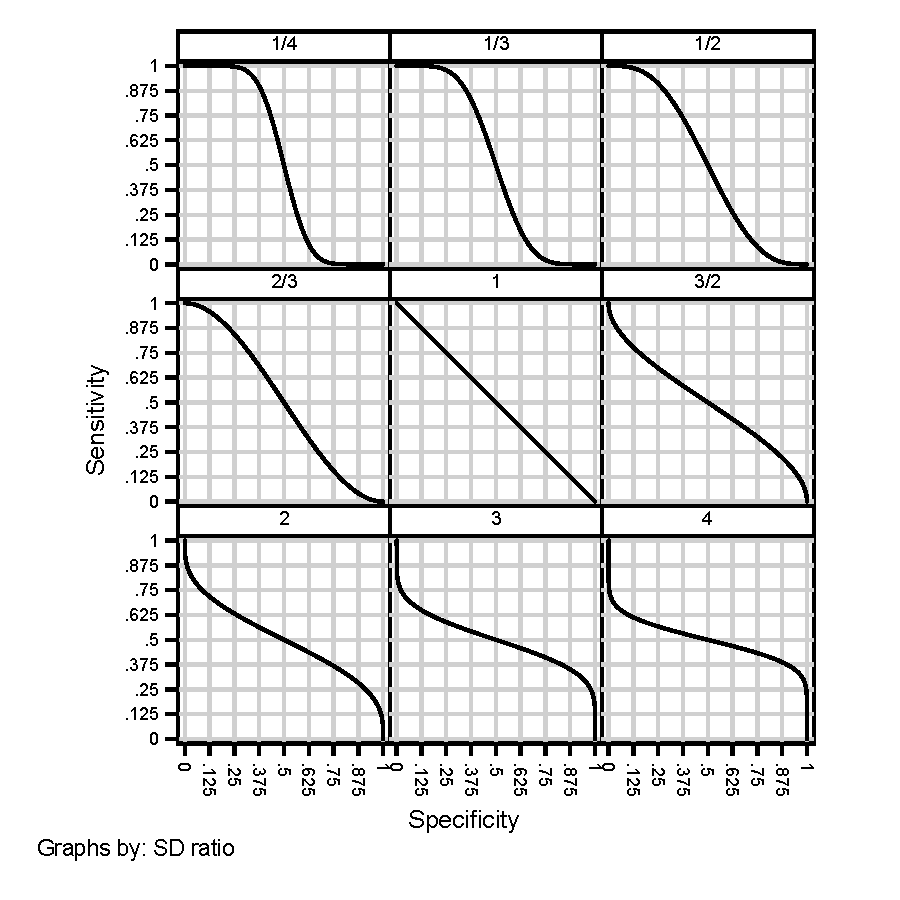
\includegraphics{senspec3.pdf}
\end{figure}

Figure~\ref{figure:figseq2} shows the sensitivity--specificity curves under 9 different SD ratios $\sigma_1/\sigma_0$,
namely 1/4, 1/3, 1/2, 2/3, 1, 3/2, 2, 3 and 4.
Again, in each subplot, we can simulate the distribution of the $\bar g_{0.5,0}(U_{0j})$
by sampling at random from the horizontal specificity axis and recording the corresponding sensitivity,
and we can simulate the distribution of the $\bar g_{0.5,1}(U_{1j})$
by sampling at random from the vertical sensitivity axis and recording the corresponding specificity.
Note that, as the SD ratio increases, the sensitivities $\bar g_{0.5,0}(U_{0j})$ become progressively less variable,
and the specificities $\bar g_{0.5,1}(U_{1j})$ become progressively more variable.
The central plot (in the second row and the second column)
gives the case where $\sigma_0=\sigma_1$,
under which conditions the two population distributions differ only in location,
and the $\bar g_{0.5,i}(U_{ij})$ are uniformly distributed over the unit interval, wtth a variance of 1/12.
The variance of $\hat\beta_{0.5,N_0,N_1}$ then converges in ratio to
\begin{equation}
{{\pi \sigma_0^2}\over{3}} \left( N_0^{-1} + N_1^{-1} \right) .
\label{eq:eqseq29}
\end{equation}
In this equal--variance case, the corresponding variance for the mean difference converges in ratio to $\sigma_0^2(N_0^{-1}+N_1^{-1})$,
implying that, \textit{if} the distributions are indeed Normal with equal variances,
\textit{then} the variance ratio between the median difference and the mean difference is the familiar $\pi/3$,
or approximately 1.0471976 (Hodges and Lehmann, 1963)\cite{hodges1963}.

\section{Differences between subpopulation percentiles}

For $i\in \{0,1\}$ and $q\in (0,1)$, a $100q$th percentile of the $Y$--values in the $i$th population $\xi_{q,i}$ is a solution in $z$
to the equation
\begin{equation}
0 \quad = \quad F_i(z) - q \quad = \quad E\left[ \, I(Y_{ij} \le z ) \, \right] - q.
\label{eq:eqseq30}
\end{equation}
$\xi_{q,i}$ is unique if $F_i(\cdot)$ is strictly monotonically increasing, and we will assume this from this point.
The sample estimate of $\xi_{q,i}$, for a sample of $N_i$, will be denoted $\hat\xi_{q,i,N_i}$,
and is calculated by substituting sample means for the population means in (\ref{eq:eqseq30}) and solving numerically in $z$.
The estimate $\hat\xi_{q,i,N_i}$ is an $M$--estimate in the terminology of Chapter~7 of Serfling (1980)\cite{serfling1980}.
Its limiting distribution as $N_i \rightarrow \infty$ is therefore defined, using the methods of that source, as follows.
The derivative with respect to $z$ of (\ref{eq:eqseq30}) is
\begin{equation}
{d\over {dz}}\left\{ E\left[ \, I(Y_{ij} \le z ) \, \right] - q \right\}
\quad = \quad {d\over {dz}}\left[ F_i(z) - q \right] \quad = \quad f_i(z).
\label{eq:eqseq31}
\end{equation}
It follows (assuming the usual regularity conditions) that the distribution of $\hat\xi_{q,i,N_i}$ tends asymptotically to a Normal form,
with mean $\xi_{q,i}$ and variance converging in ratio to
\begin{equation}
\left[ f_i(\xi_{q,i}) \right]^{-2} V\left[ \, \#\{ j: 1\le j \le N_i, Y_{ij} \le \xi_{q,i} \} /N_i - q \, \right]
\quad = \quad \left[ f_i(\xi_{q,i}) \right]^{-2} {{q(1-q)}\over{N_i}},
\label{eq:eqseq32}
\end{equation}
where $\#S$ denotes the cardinality of a set $S$.
Therefore, by the rules governing variances of linear combinations of independent variables,
the difference $\hat\xi_{q,1,N_1} - \hat\xi_{q,0,N_0}$ between the sample percentiles
has a sampling distribution tending to an asymptotically Normal form,
with mean $\xi_{q,1} - \xi_{q,0}$ and variance converging in ratio to
\begin{equation}
\left[ f_0(\xi_{q,0}) \right]^{-2} N_0^{-1} q(1-q) \quad + \quad \left[ f_1(\xi_{q,1}) \right]^{-2} N_1^{-1} q(1-q).
\label{eq:eqseq33}
\end{equation}
This equation can be used in approximate power and sample size calculations,
if we have expressions for the $f_i(\cdot)$.
Bonett and Price (2002)\cite{bonett2002} discuss the problems involved in doing this,
with the general linear function of subpopulation medians ($q=0.5$).
In general, it is usual to assume a model for these power calculations,
as it is with power calculations involving the variances of Hodges--Lehmann median differences,
specified by (\ref{eq:eqseq27}).
In both cases, a squared inverse density function is involved,
and this squared inverse density function may be sensitive to model assumptions.

\subsection{Median differences \textit{versus} differences between medians}

In general, a Hodges--Lehmann percentile difference is \textit{not} the same parameter as a difference between percentiles.
Methods for estimating the two classes of parameters should be viewed as methods for estimating alternative parameters,
and \textit{not} as alternative methods for estimating the same parameter.
A counterexample in the case of medians is the case where the two subpopulations are exponential, with different hazard rates.
In that case, the Hodges--Lehmann median difference has a lower absolute value than the difference between medians,
which in turn has a lower absolute value than the difference between means.
This is discussed in Newson (2008)\cite{newson2008}.

\textit{However}, the two parameters may be the same if the parameter is a median ($q=0.5$),
and if, in addition, the two subpopulation distributions either are both symmetrical around their respective medians,
or differ only in location, or both.
If either of these conditions is even approximately true,
then there may be a perception that the two parameters are measuring something similar.
Under these circumstances, we may ask whether we gain or lose power to detect a population difference
by estimating median differences instead of differences between medians, or \textit{vice versa}.

Note from (\ref{eq:eqseq27}) and (\ref{eq:eqseq33})
that the asymptotic variance formulas for median differences and differences between medians both resolve into a sum of two terms,
one corresponding to each sample.
Each of these terms in turn resolves into 3 factors.
The first factor is an inverse squared density function,
derived either from one of the $f_i(\cdot)$ or from $f_\Delta(\cdot)$.
The second factor is the reciprocal of the subsample number, and is the same for corresponding terms in both expressions.
The third factor is a variance,
which, in the case of a difference between medians, is the Bernoulli variance $q(1-q)=0.5(1-0.5)=0.25$,
and, in the case of a median difference, is the variance of a continuous variable bounded between 0 and 1.
As the second factor (the reciprocal of the subsample number) is the same for corresponding terms in both expressions,
any advantage of a lower variance for either one parameter or the other
must arise from the first factor (the inverse squared density)
or from the third factor (the variance).

For a median, the third factor (the variance factor) cannot possibly be larger for the median difference than for the difference between medians.
This is because, in this case, the variance factor for the difference between medians belongs to a Bernoulli variable,
which has mean 0.5, but which can either be 0 or 1,
whereas the variance factor for the median difference belongs to a continuous variable $\bar g_{0.5,i}(U_{ij})$,
bounded between 0 and 1, with the same mean.
The continuous variable will therefore always be no further from its mean than the Bernoulli variable,
and may be considerably closer to its mean.
The variance factor therefore favors median differences over differences between medians.

The first factor (the inverse squared density) will \textit{usually} be higher for a difference between medians than for a median difference.
This is because, in the case of a difference between medians,
the density belongs to the original $Y$--variable in one of the two subpopulations,
whereas, in the case of a median difference,
the density belongs to a difference between two independently--sampled $Y$--values,
one from each subpopulation.
This difference will have a variance equal to the sum of the two subpopulation variances,
if the variance of the difference exists at all.
Distributions with higher variances usually (but not always) have higher densities at their medians than distributions with lower variances.
Therefore, the inverse squared density factor will probably favor differences between medians over median differences.

Four simple examples of ``toy models'' are the homoskedastic Normal, the homoskedastic shifted exponential,
the homoskedastic shifted Laplace (or shifted double--exponential), and the homoskedastic Cauchy.
In all of these models, the two subpopulation distributions differ only in location,
implying that the distributions of the $\bar g_{0.5,i}(U_{ij})$ will be uniform over the unit interval,
with a common variance of 1/12,
and also that the subpopulation densities will be equal at their respective medians.
The asymptotic ratio between the variance of the difference between medians and the variance of the median difference
will therefore be equal to
\begin{equation}
{{ 12 f_0(\xi_{0.5,0})^{-2} }\over{ 4f_\Delta(\beta_{0.5})^{-2} }} \quad = \quad {{3f_\Delta(\beta_{0.5})^2}\over{f_0(\xi_{0.5,0})^{2}}}.
\label{eq:eqseq34}
\end{equation}
This implies that the squared density of the subpopulation distributions at their medians
must be at least 3 times the squared density of the pairwise difference distribution at its median,
in order for the difference between medians to be no more variable than the median difference.

In the case of the homoskedastic Normal model,
$f_\Delta(\cdot)$ is a Normal density, with twice the variance of the $f_i(\cdot)$,
so the squared density ratio is 2.
In the case of the homoskedastic shifted exponential model,
$f_\Delta(\cdot)$ is a shifted Laplace density, with the same hazard rate as the $f_i(\cdot)$,
so the squared density ratio is 1.
\textit{However}, in the case of the homoskedastic shifted Laplace model,
each of the $f_i(\cdot)$ belongs to a two--way equal mixture of a shifted positive exponential and a shifted negative exponential,
implying that $f_\Delta(\cdot)$ belongs to a 4--way equal mixture of a shifted positive exponential, a shifted negative exponential,
a shifted positive Gamma with the same limiting hazard rate and an inverse squared coefficient of variation of 2,
and a shifted negative Gamma with the same limiting hazard rate and an inverse squared coefficient of variation of 2.
This in turn implies that the density $f_\Delta(\cdot)$ at its median is half the density of the $f_i(\cdot)$ at their medians,
giving a squared density ratio of 4.
Similarly, in the case of the homoskedastic Cauchy model,
$f_\Delta(\cdot)$ belongs to a Cauchy distribution with a scale parameter twice that of the $f_i(\cdot)$,
implying half the density at its median, and therefore a squared density ratio of 4.
\textit{Therefore}, the variance of the median difference is 2/3 of the variance of the difference between medians in the homoskedastic Normal case,
is 1/3 of the variance of the difference between medians in the homoskedastic shifted exponential case,
but is 4/3 of the variance of the difference between the medians in the homoskedastic shifted Laplace and homoskedastic Cauchy cases.
This implies that, even when the median difference \textit{is} the difference between the medians,
this parameter may be estimated more or less efficiently (depending on the model)
by using a confidence interval for a median difference
than by using a confidence interval for a difference between medians.

The choice betwen these two methods is therefore not a simple subject.
\textit{However}, the formulas in this document can enable the numerical investigation
of more complicated cases than these.

{\parindent=0pt

\smallskip

\begin{thebibliography}{10}

\bibitem{bonett2002}
Bonett DG, Price RM.
Statistical inference for a linear function of medians:
Confidence intervals, hypothesis testing, and sample size requirements.
\textsl{Psychological Methods} 2002; \textbf{7(3)}: 370--383.

\bibitem{edwardes1995}
Edwardes, M. D. d. B. A confidence interval for $\Pr(X<Y)-\Pr(X>Y)$ estimated from simple cluster samples.
\textsl{Biometrics} 1995; \textbf{51(2)}: 571�-578.

\bibitem{hanley1982}
Hanley JA, McNeil BJ.
The meaning and use of the area under a receiver operating characteristic (ROC) curve.
\textsl{Radiology} 1982; \textbf{143(1)}: 29-�36.

\bibitem{harrell1982}
Harrell FE, Califf RM, Pryor DB, Lee KL, Rosati RA.
Evaluating the yield of medical tests.
\textsl{Journal of the American Medical Association} 1982; 247(18): 2543�-2546.

\bibitem{hodges1963}
Hodges JL, Lehmann EL. Estimates of location based on rank tests.
\textsl{The Annals of Mathematical Statistics} 1963; \textbf{34(2)}: 598--611.

\bibitem{lehmann1963}
Lehmann EL. Nonparametric confidence intervals for a shift parameter.
\textsl{The Annals of Mathematical Statistics} 1963; \textbf{34(4)}: 1507--1512.

\bibitem{newson2002}
Newson R. Parameters behind ``nonparametric'' statistics: Kendall's tau, Somers'~$D$ and median differences.
\textsl{The Stata Journal} 2002; \textbf{2(1)}: 45--64.

\bibitem{newson2004}
Newson R. Generalized power calculations for generalized linear models and more.
\textsl{The Stata Journal} 2004; \textbf{4(4)}: 379--401.

\bibitem{newson2006}
Newson R. Confidence intervals for rank statistics: Percentile slopes, differences, and ratios.
\textsl{The Stata Journal} 2006; \textbf{6(4)}: 497--520.

\bibitem{newson2008}
Newson RB. Hodges-Lehmann median differences between exponential subpopulations. 12~October, 2008.
Downloadable from
\href{http://www.imperial.ac.uk/nhli/r.newson/papers.htm}{\textsl{http://www.imperial.ac.uk/nhli/r.newson/papers.htm}}
as of 17~June, 2009.

\bibitem{serfling1980}
Serfling RJ. Approxination Theorems of Mathematical Statistics.
New York, NY: John Wiley \& Sons; 1980.

\bibitem{somers1962}
Somers RH. A new asymmetric measure of association for ordinal variables.
\textsl{American Sociological Review} 1962; \textbf{27(6)}: 799-�811.

\end{thebibliography}

}

\end{document}               % End of document.
